\chapter{Revisión de técnicas}
En este capítulo se describen las técnicas y algoritmos que preceden y en los que se basa el trabajo descrito en esta memoria. Concretamente, se realiza una introducción a las redes neuronales y \textit{Deep Learning}, tras la cual se habla de los principales métodos de aprendizaje por refuerzo clásicos y actuales. Finalmente, se estudian algunos de los principales algoritmos de navegación autónoma existentes.

\section{Redes neuronales y \textit{Deep Learning}}

En esta sección se describe el concepto de las redes neuronales y sus principales características. Tras esto, se describe \textit{Deep Learning} y uno de sus modelos más característicos, las redes convolucionales.

\subsection{Redes neuronales}
En el campo de la inteligencia artificial, una \textbf{neurona} (también conocida como \textbf{nodo}) es la unidad lógica básica que forma una red neuronal \cite{alma991004256519704990}. En esencia, una neurona es una función matemática no lineal que, a partir de unas entradas, genera una salida. Además, las neuronas se conectan entre ellas a través de conexiones dirigidas, por lo que se puede propagar esta salida entre ellas.

La estructura básica de una neurona se puede observar en la Figura \ref{fig:chap3-neuron}, siendo los componentes principales \cite{alma991004256519704990}:

\begin{figure}[h]
    \centering
    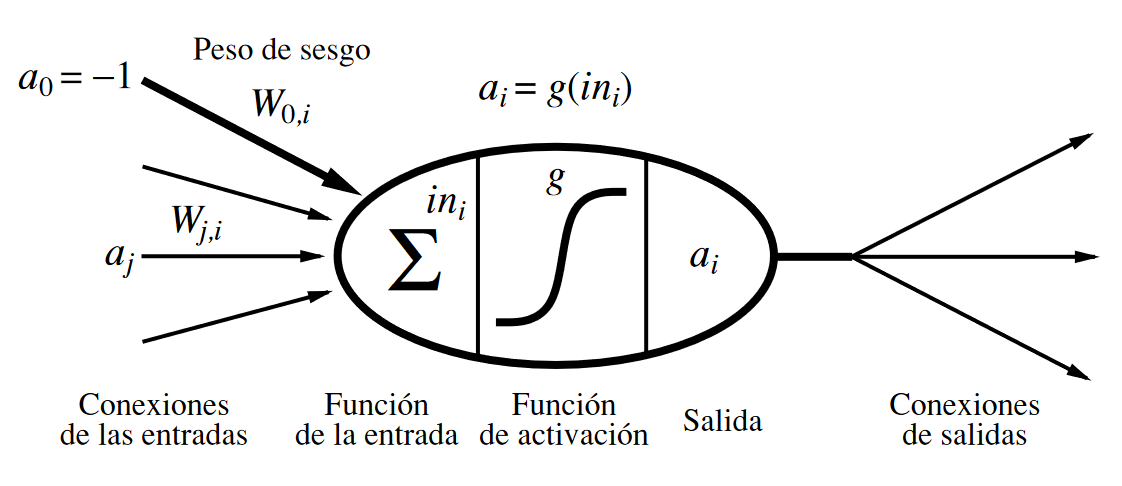
\includegraphics[width=0.7\textwidth]{imagenes/cap3/neuron.png}
    \caption{Estructura de una neurona artificial \cite{alma991004256519704990}.}
    \label{fig:chap3-neuron}
\end{figure}

\begin{itemize}
	\item \textbf{Conexiones de las entradas:} El conjunto de entradas recibidos por la neurona. Estas entradas $a_j$ están ponderadas por pesos $w_{j,i}$ (siendo $i$ la neurona actual y $j$ el origen de la entrada) determinando el peso y el signo de cada entrada.
	\item \textbf{Función de entrada:} La función de entrada $in_i$ no es más que el sumatorio de todas las entradas ponderadas que recibe la función, siendo éste:
	\[in_i=\sum_{j=0}^N w_{j,i}a_j\]
Donde $N$ es el número total de entradas.
	\item \textbf{Función de activación:} La función de activación $g$ es una función aplicada a la función de entrada para generar la salida $a_i$. Esta función debe cumplir que:
	\begin{itemize}
		\item La función debe devolver valores adecuados (la neurona debe estar activa o con una salida cercana a $+1$ con las entradas correctas y apagada o con salida cercana a $0$ en otro caso).
		\item La función debe ser no lineal para evitar que toda la red neuronal se pueda simplificar a una función lineal simple \cite{alma991004256519704990}.
	\end{itemize}
	Hay varias funciones de activación usadas, siendo algunas de las más comunes la función umbral o la lineal. Ahora bien, la función más típica es la \textbf{función sigmoide}, teniendo ésta la fórmula:
	\[g(in_i)=\frac{1}{1+e^{-in_i}}\]
	\item \textbf{Salida:} La salida $a_i$ no es más que la aplicación de la función de activación sobre la función de entrada, $a_i = g(in_i)$. Esta salida se puede propagar a otras neuronas (siendo ésta una de las entradas de dichas neuronas), o servir como salida de la red neuronal.
\end{itemize}

	Como se puede ver en la Figura \ref{fig:chap3-neuron}, las neuronas tienen una entrada constante $a_0$ conocida como la entrada de sesgo, de valor $a_0 = -1$, cuyo peso se conoce como el \textbf{peso de sesgo}. La utilidad de este peso es definir el umbral real de la neurona (es decir, una neurona se activa únicamente cuando la suma de todas las entradas supera a este peso de sesgo) \cite{alma991004256519704990}. El peso de sesgo permite desplazar la activación de la neurona sin alterar la pendiente, de forma similar al término independiente de una recta.
	
Definida una neurona, se puede definir una \textbf{red neuronal artificial} como un grupo de neuronas trabajando en conjunto, representando una función compleja no lineal con una gran cantidad de parámetros (los pesos de sus neuronas). \cite{alma991004256519704990}. Existen dos tipos de redes neuronales: redes cíclicas o \textbf{recurrentes} y redes acíclicas o de \textbf{propagación hacia adelante} \cite{alma991004256519704990}, siendo éstas el foco de esta sección.

Una \textbf{red neuronal de propagación hacia adelante} es una red acíclica de neuronas representando una función a partir de las entradas de la red, sin ningún tipo de estado interno o memoria \cite{alma991004256519704990}. Este tipo de redes suele estar organizado en \textbf{capas}, siendo una capa un conjunto de neuronas de forma que una neurona recibe únicamente entradas de la capa anterior y propaga sus entradas únicamente a la capa posterior \cite{alma991004256519704990}. Dependiendo del número de capas, se puede hablar de redes de una única capa (\textbf{perceptrones}) o de redes de varias capas (\textbf{perceptrones multicapa} o \textit{MLPs}) \cite{alma991004256519704990}.

Un \textbf{perceptrón multicapa} es la estructura más típica de red neuronal de propagación hacia adelante, siendo ésta una red neuronal con más de una capa \cite{alma991004256519704990}, teniendo cada capa un número variable de neuronas. La principal ventaja de este tipo de estructura es su capacidad de (con un número suficiente de neuronas) aproximar cualquier función no lineal \cite{Goodfellow-et-al-2016}. Se puede observar un ejemplo de perceptrón multicapa en la Figura \ref{fig:chap3-mlp}, viendo que la estructura se divide en tres partes \cite{10.5555/3161223}:

\begin{itemize}
	\item \textbf{Capa de entrada:} Representa las entradas de la red (las entradas de la función a simular). Es típico que estas neuronas no usen una función de activación.
	\item \textbf{Capa(s) oculta(s):} Una o más capas ubicadas entre las capas de entrada y salida. Estas capas se encargan de identificar las relaciones existentes entre las entradas durante el entrenamiento \cite{10.5555/3161223}, para obtener la salida esperada.
	\item \textbf{Capa de salida:} Representa las salidas finales procesadas de la red (las salidas de la función a aproximar).
\end{itemize}

\begin{figure}[h]
    \centering
    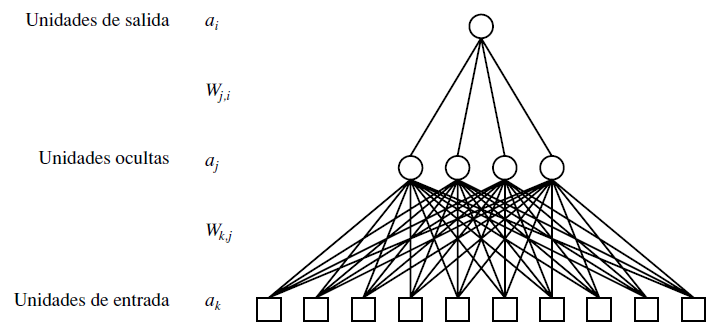
\includegraphics[width=0.7\textwidth]{imagenes/cap3/mlp.png}
    \caption{Perceptrón multicapa con una capa oculta \cite{alma991004256519704990}.}
    \label{fig:chap3-mlp}
\end{figure}

El principal objetivo a la hora de desarrollar una red neuronal es encontrar el conjunto de pesos que logre que, para unos valores de entrada, la salida de la red neuronal se aproxime lo máximo posible al comportamiento esperado en el problema real \cite{Zhang2003ArtificialNN}. Esto se consigue \textbf{entrenando} la red neuronal a partir de un conjunto de entrenamiento (cuyos valores de salida son conocidos), utilizando el algoritmo de \textbf{retropropagación} (propuesto originalmente por Rumelhart \textit{et al.} en 1986 \cite{Rumelhart:1986we}). El objetivo del algoritmo es ajustar los pesos de la capa de salida para minimizar el error, y posteriormente propagar este ajuste a las capas anteriores para ajustar sus pesos usando gradiente descendiente, con el objetivo de minimizar el error de la red. 

El pseudocódigo del algoritmo se puede ver en la Figura \ref{alg:chap3-back}. Por lo general, la condición de parada del algoritmo de retropropagación consiste en alcanzar un umbral de error o realizar el proceso un número determinado de veces sobre el conjunto de entrenamiento entero. Cada ciclo del algoritmo sobre el conjunto de entrenamiento completo se conoce como una \textbf{época} (o \textit{epoch} por su nombre en inglés) \cite{alma991004256519704990}. 

\begin{figure}
\begin{algorithm}[H]
\SetAlgorithmName{Algoritmo}{algoritmo}{Lista de algoritmos}
\caption{Algoritmo de retropropagación}
\textbf{Variables iniciales:} Conjunto de entrenamiento $ent$, formado por tuplas de elementos $(x, y)$ (siendo $x$ las entradas de la red y $y$ las salidas esperadas de la red). Pesos de la red neuronal $w_{i,j}$ donde $i,j$ indica un peso dirigido de la neurona $i$ a la neurona $j$.\\
\textbf{1.} Inicializa los pesos de la red neuronal utilizando valores aleatorios.\\
\textbf{2.} Mientras no se cumpla la condición de parada:\\
\Indp \textbf{2.1.} Para cada ejemplo $(x, y)$ contenido en el conjunto de entrenamiento $ent$:\\
\Indp \textbf{2.1.1.} Calcula la salida $h_N$ para todas las neuronas $N$ de la red neuronal, utilizando propagación hacia adelante.\\
\textbf{2.1.2.} Calcula el error $error$, las salidas obtenidas $h_N$ y las salidas esperadas $y_N$ para cada neurona $N$.\\
\textbf{2.1.3.} Para cada neurona $N$ (empezando por las neuronas de la capa de salida, y retrocediendo en orden hasta la capa de entrada):\\
\Indp \textbf{2.1.3.1.} Calcula la influencia de la neurona $N$ en el error final, $\delta_N$:\\
Si $N$ es una neurona de salida:
\[\delta_N = (y_N - h_N) * h_N * (1-h_N)\]\\
En otro caso ($N$ pertenece a una capa oculta):
\[\delta_N = \left(\sum_{X \in sucesores(N)} w_{N,X} * \delta_X \right) * h_N *(1-h_N)\]
Donde $sucesores(N)$ es un conjunto de las neuronas en la capa posterior a la capa de la neurona $N$.\\
\textbf{2.1.3.2.} Para todas las neuronas $R$ pertenecientes a la capa anterior a la capa de la neurona $N$, calcula la actualización $\Delta_{R,N}$:
\[\Delta_{R,N} = \eta * \delta_N * h_R\]
Donde $\eta$ es el factor de aprendizaje de la red neuronal.\\
\Indm \textbf{2.1.4.} Para cada peso $w_{R,N}$ en la red neuronal, actualiza el peso:
\[w_{R,N} = w_{R,N} + \Delta_{R,N}\]\\
\Indm \Indm \textbf{3.} \textbf{Devolver} la red con los pesos entrenados.
\end{algorithm}
\hrule
\caption{Algoritmo de retropropagación para entrenamiento de perceptrones multicapa.}
\label{alg:chap3-back}
\end{figure}

\subsection{Aprendizaje por representación y \textit{Deep Learning}}

El \textbf{aprendizaje por representación} es un conjunto de métodos contenidos dentro del aprendizaje automático cuyo objetivo es, dada una entrada sin procesar, extraer las características más relevantes de la entrada para trabajar con ellas \cite{Goodfellow-et-al-2016}. Esto permite resolver uno de los problemas más típicos del aprendizaje automático, determinar las características más relevantes de un problema. Ahora bien, los algoritmos pueden tener problemas para extraer directamente características abstractas de alto nivel (como los contornos de un objeto o los acentos de una voz). 

Para solucionar este problema surge \textbf{\textit{Deep Learning}}, un subconjunto de las técnicas de aprendizaje por representación que utilizan varios niveles de abstracción, partiendo de conceptos básicos que van componiendo para alcanzar conceptos complejos y abstractos \cite{Goodfellow-et-al-2016}. La principal ventaja frente a otros métodos es que estas características son identificadas automáticamente por los algoritmos, sin necesidad de un experto que guíe el aprendizaje.

Actualmente, las técnicas de \textit{Deep Learning} se han vuelto el estado del arte en una gran cantidad de problemas que se consideraban inabordables hace apenas una década, como la visión artificial, el reconocimiento de voz o el procesamiento de lenguaje natural \cite{Goodfellow-et-al-2016} entre otros.

La familia de modelos más característica de \textit{Deep Learning} es las redes neuronales, siendo uno de los modelos más usados los perceptrones multicapa descritos previamente \cite{Goodfellow-et-al-2016}. Estas redes se conocen también como \textbf{redes neuronales profundas}, teniendo éstas una gran cantidad de capas ocultas y neuronas por capa (donde cada capa se encarga de aprender un nivel de representación de la entrada).

Ahora bien, el aumento del tamaño de las redes neuronales profundas (tanto en neuronas como en capas) conlleva una serie de problemas:

\begin{itemize}
	\item Conforme aumenta el tamaño de la red, aumenta el número de parámetros (pesos) a ajustar. Esto significa que se necesitan conjuntos de entrenamiento exponencialmente más grandes para alcanzar buenos resultados y, por tanto, un mayor coste computacional y de tiempo para el entrenamiento.
	
	Esto se ha solucionado principalmente mediante el uso de ordenadores más potentes, conjuntos de datos más grandes y técnicas para ampliar los conjuntos de datos ya existentes como el \textit{data augmentation} \cite{Shorten2019ASO}. 
	
	\item \textbf{Problema del gradiente desvaneciente / explosivo (\textit{Vanishing / Exploding gradient problem):}} Al aumentar el número de capas, la eficiencia del algoritmo de retropropagación disminuye si se utilizan las funciones de activación tradicionales (como la función sigmoide) \cite{gradientKolen}. Esto se debe a que la propagación del error puede diluirse (provocando cambios demasiado lentos) o incrementar rapidamente (provocando inestabilidad) conforme se propaga de capa en capa.
	
	Una de las principales soluciones al problema es el uso de funciones de activación específicas como \textit{ReLU} \cite{Goodfellow-et-al-2016}, siendo la fórmula:
	\[g(in_i)=max\{0,in_i\}\]
\end{itemize}

Si bien las redes neuronales profundas son uno de los modelos más usados en \textit{Deep Learning}, también es frecuente el uso de otros tipos de redes neuronales como redes recurrentes, redes recursivas, redes residuales... o redes convolucionales, como se verán a continuación \cite{Goodfellow-et-al-2016}.

\subsection{Redes neuronales convolucionales}

Una \textbf{red neuronal convolucional} es una red neuronal que usa funciones de convolución, diseñada para trabajar con entradas en forma de matrices (como líneas de tiempo o imágenes) \cite{Goodfellow-et-al-2016}. Éstas fueron originalmente propuestas por Yann LeCun \textit{et al.} en 1989 \cite{10.1162/neco.1989.1.4.541}, si bien cobraron importancia tras \textit{AlexNet} \cite{Krizhevsky2012ImageNetCW} y sus resultados en la competición de \textit{ImageNet}.

En el campo del aprendizaje automático, una \textbf{convolución} es una operación matemática lineal aplicada sobre dos funciones de números reales: una \textbf{entrada (\textit{input})} $I$, generalmente una matriz de datos como puede ser una imagen; y un \textbf{nucleo (\textit{kernel})} $K$, una matriz de parámetros entrenables. La salida de esta operación es otra matriz, típicamente conocida como el \textbf{mapa de características (\textit{feature map})} $S$ \cite{Goodfellow-et-al-2016}. Esta función normalmente se define como:
\[S(i,j)=(K*I)(i,j)=\sum_m \sum_n I(i-m,j-n)K(m,n)\]
Donde $m$ y $n$ son las dimensiones del núcleo. Se puede ver un ejemplo de la función actuando sobre una entrada con un núcleo en la Figura \ref{fig:chap3-conv}.
\begin{figure}[h]
    \centering
    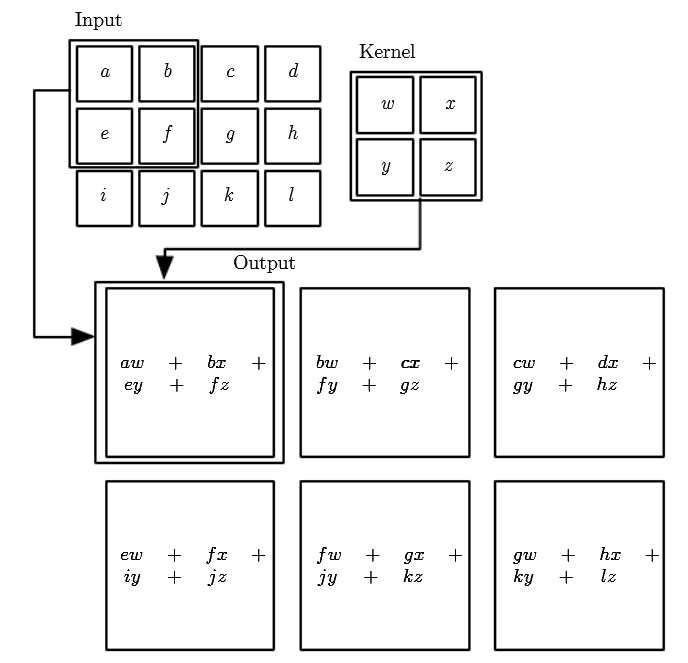
\includegraphics[width=0.7\textwidth]{imagenes/cap3/conv.png}
    \caption{Ejemplo de operación de convolución \cite{Goodfellow-et-al-2016}.}
    \label{fig:chap3-conv}
\end{figure}

Normalmente, se suelen utilizar \textbf{varios \textit{kernels}} en vez de uno único, permitiendo detectar varias características a partir de una misma entrada \cite{10.5555/3161223}. Esto hace que el mapa de características obtenido como resultado pase a ser una matriz tridimensional (donde cada capa representa los resultados de uno de los filtros).

El uso de convoluciones en las redes neuronales ofrece ventajas significativas  respecto a las redes neuronales profundas tradicionales \cite{Goodfellow-et-al-2016}:
\begin{itemize}
	\item \textbf{Conectividad dispersa:} En las redes neuronales profundas, es normal que una neurona de una capa reciba entradas de todas las neuronas de la capa anterior, y propague su salida a todas las neuronas de la capa posterior. Esto puede provocar que el número de parámetros a ajustar crezca exponencialmente para entradas grandes y redes con muchas capas y neuronas \cite{10.5555/3161223}.
	
	En cambio, el uso de convolución con \textit{kernels} más pequeños que la entrada reduce drásticamente el número de conexiones, aumentando la eficiencia.
	\item \textbf{Parámetros compartidos:} En redes neuronales profundas estándares, cada parámetro (peso) interactúa únicamente en una propagación (el peso $w_{i, j}$ solo es relevante para la propagación entre las neuronas $i$ y $j$).
	
	En cambio, cada parámetro del \textit{kernel} interactúa con todos los valores de la entrada, reduciendo el número de parámetros que necesitan ser entrenados en la red, acelerando el entrenamiento.
	\item \textbf{Representación equivariante:} La convolución es \textbf{equivariante}, lo que significa que cualquier cambio en la entrada se refleja de forma idéntica en su representación en el mapa de características.
	
	Esto permite, por ejemplo, que si en una imagen de entrada se desplaza un objeto, su representación en la salida se verá desplazada de forma equivalente, permitiendo una mayor generalización a la hora de detectar características.
\end{itemize}

Por lo general, una capa de convolución en una red neuronal convolucional tiene la siguiente estructura \cite{Goodfellow-et-al-2016}: 
\begin{enumerate}
	\item Una \textbf{convolución} con una entrada y varios núcleos, como se ha descrito previamente.
	\item Una \textbf{función de activación} aplicada sobre el mapa de características obtenido de la convolución. Generalmente se utiliza \textit{ReLU}.
	\item Una función de \textbf{\textit{pooling}}. Una función de \textit{pooling} es una función matemática similar a la convolución que sustituye una región de la red de tamaño $(m,n)$ por un único estadístico de los valores de la región. Ésto se realiza principalmente para reducir el tamaño de la salida (permitiendo encadenar más convoluciones) y para mejorar la capacidad de invariancia de la convolución.
	
	Generalmente, el estadístico más utilizado para la función de \textit{pooling} es el \textbf{máximo} \cite{Zhou1988ComputationOO}, aunque también es común utilizar la \textbf{media}. Se puede ver un ejemplo de una operación de \textit{pooling} por máximo en la Figura \ref{fig:chap3-pool}.
\end{enumerate}

\begin{figure}[h]
    \centering
    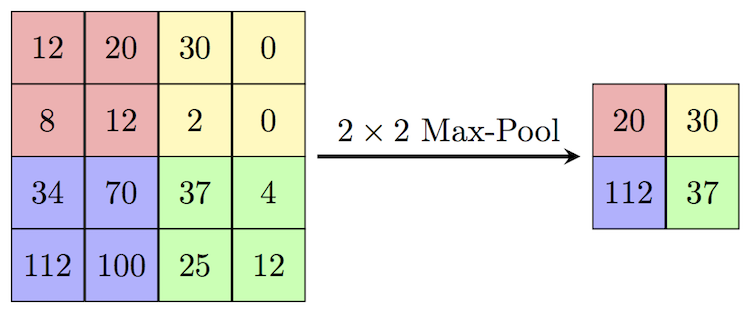
\includegraphics[width=0.7\textwidth]{imagenes/cap3/pooling.png}
    \caption{Ejemplo de \textit{pooling} usando estadístico de máximo \cite{cswiki18}.}
    \label{fig:chap3-pool}
\end{figure}




\section{Aprendizaje por refuerzo}

El \textbf{aprendizaje por refuerzo} es un subconjunto de métodos de aprendizaje automático consistentes en enseñar a un agente a actuar de forma óptima en cada situación para maximizar una recompensa numérica \cite{Sutton1998}.

Existen dos características principales que distinguen al aprendizaje por refuerzo de otros métodos de aprendizaje automático (como el aprendizaje supervisado o el no supervisado) \cite{Sutton1998}:
\begin{itemize}
	\item El agente no conoce de antemano las acciones óptimas, sino que debe descubrirlas mediante ensayo y error.
	\item Las acciones del agente no solo afectan a la recompensa inmediata, sino que pueden afectar a los estados y recompensas futuras.
\end{itemize}

Los dos componentes principales de un problema de aprendizaje por refuerzo son el \textbf{agente} (encargado de aprender y tomar decisiones) y el \textbf{entorno} (todo lo que no es el agente, con lo que interactúa) \cite{Sutton1998}. Además, en la relación entre estos dos componentes se pueden encontrar tres conceptos cuya definición adecuada es necesaria para la resolución correcta del problema \cite{Sutton1998}:
\begin{itemize}
 \item \textbf{Estado ($s$):} Una representación del estado actual del entorno, tal cual lo interpreta el agente. Esta representación $s_t$ pertenece a un conjunto de estados $S$.
 
 La definición del estado debe cumplir la \textbf{Propiedad de Markov:} el estado, por sí mismo, debe ser capaz de representar toda la información relevante \cite{Sutton1998}. Esto significa que el estado que se alcance tras realizar una acción debe depender únicamente del estado actual, y no de ningún estado o acción previa.
 \item \textbf{Acción ($a$):} Una actuación llevada a cabo por el agente según el estado actual $s_t$. Una acción $a_t$ pertenece a un conjunto posible de acciones en un estado concreto, $A(s)$.
 \item \textbf{Recompensa ($r$):} Un valor numérico positivo (recompensa) o negativo (penalización) otorgada por el entorno tras la actuación del agente. El objetivo del agente a largo plazo es \textbf{maximizar la recompensa obtenida}.
 
 El principal objetivo de las recompensas es formalizar la meta del agente. Es decir, un agente que maximiza las recompensas debería ser un agente que alcanza la meta propuesta.
\end{itemize}

El agente y el entorno interactúan en un bucle continuo como se puede ver en la Figura \ref{fig:chap3-rl}, donde en cada paso $t$ \cite{Sutton1998}:

\begin{figure}[h]
    \centering
    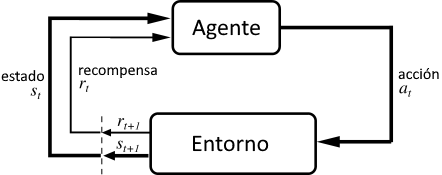
\includegraphics[width=0.7\textwidth]{imagenes/cap3/rl.png}
    \caption{Interacción entre agente y entorno en el aprendizaje por refuerzo \cite{Sutton1998}.}
    \label{fig:chap3-rl}
\end{figure}

\begin{enumerate}
\item El agente percibe un estado $s_t$ del entorno.
\item El agente procesa el entorno y elige una acción $a_t$, que aplica sobre el entorno.
\item El entorno se modifica como respuesta a la acción $a_t$ y devuelve al agente un nuevo estado $s_{t+1}$, junto a la recompensa obtenida $r_{t+1}$.
\end{enumerate}

Además del agente y el entorno, hay otros cuatro conceptos de gran importancia en la definición de un problema de aprendizaje por refuerzo \cite{Sutton1998}:

\begin{itemize}
\item \textbf{Política $(\pi)$:} Método de actuación de un agente ante un estado $s$ en un instante concreto, definiéndose como una función $\pi(s) = a$. La política es uno de los puntos claves del aprendizaje automático, siendo el objetivo a optimizar y pudiendo determinar la actuación del agente por sí misma.
\item \textbf{Modelo:} Representación aproximada del entorno y su comportamiento usada por el agente para predecir estados y recompensas del entorno ante una acción. Este concepto es opcional, no siendo usado por todos los métodos de aprendizaje por refuerzo.
\item \textbf{Modelo de recompensas ($R(s)$ / $R(s,a)$):} Función que, para un estado $s$ (o un par estado-acción $s, a$) devuelve la recompensa adecuada al agente. Este modelo es parte del entorno y asocia a cada estado su deseabilidad inmediata (teniendo los estados deseables una recompensa mayor a los que no lo son).

Este modelo no puede ser alterado por el agente, si bien la política del agente suele alterarse como respuesta al modelo de recompensas.

\item \textbf{Modelo de utilidad ($V(s)$ / $Q(s,a)$):} Función que, para un estado $s$ (o un par estado-acción $s,a$), devuelve la \textbf{utilidad} de ese estado. En aprendizaje por refuerzo se entiende la utilidad de un estado $s$ como la recompensa total que el agente puede esperar conseguir si el estado inicial es $s$. A diferencia de las recompensas (que determinan la deseabilidad inmediata), la utilidad de un estado determina la deseabilidad a largo plazo.
\end{itemize}

En general, el objetivo principal de los algoritmos de aprendizaje por refuerzo es encontrar una política $\pi^*$ (política óptima) que maximice la utilidad de todos los estados $s$ del entorno, $V^*(s)$.

\subsection{Métodos de aprendizaje por refuerzo clásicos}

Los métodos de aprendizaje por refuerzo clásicos más usados suelen basarse en los principios del \textbf{aprendizaje por diferencia temporal} (\textit{TD-Learning}) \cite{Sutton1998}. Los modelos de esta familia son capaces de aprender directamente de las experiencias sin necesidad de estimar un modelo. Además, pueden actualizar las estimaciones de la utilidad de los estados tras cada paso realizado, pudiendo actualizar su política de forma incremental.

Se pueden distinguir dos aproximaciones a los modelos de aprendizaje por refuerzo de \textit{TD-Learning} \cite{Sutton1998}:

\begin{itemize}
\item \textbf{Métodos \textit{on-policy}:} Se optimiza la misma política que se usa para elegir la acción a realizar.
\item \textbf{Métodos \textit{off-policy}:} La política que se optimiza y la política que se usa para elegir las acciones a realizar no son la misma.
\end{itemize}

A continuación, se describen algunos de los principales métodos de aprendizaje por refuerzo usados.

\subsubsection{Q-Learning}

\textbf{Q-Learning}, propuesto originalmente por Christopher Watkins en 1989 \cite{qlearning} es un método de aprendizaje por refuerzo \textit{off-policy}, siendo el método de aprendizaje por refuerzo más importante de la época \cite{Sutton1998}.

En esencia, la actualización de la estimación de la utilidad de un par estado-acción $\hat{Q}(s_t,a_t)$ se calcula usando la siguiente fórmula \cite{Sutton1998}:
\[\hat{Q}(s_t,a_t) \leftarrow \hat{Q}(s_t,a_t) + \alpha [r_{t+1} + \gamma \max_{a'} \hat{Q}(s_{t+1},a') - \hat{Q}(s_t,a_t)]\]
Donde $\alpha$ representa el peso del nuevo valor de $\hat{Q}$, y $\gamma$ representa la depreciación realizada al estado futuro.

\textit{Q-Learning} intenta aproximar directamente la política que optimiza la utilidad, $Q^*$ independientemente de la política que se esté utilizando gracias al operador de máximo \cite{Sutton1998}, obteniendo la máxima utilidad del estado alcanzado. Esto convierte a \textit{Q-Learning} en un método \textit{off-policy} como se ha comentado previamente.

Se puede observar el pseudocódigo del algoritmo en la Figura \ref{alg:chap3-qlearning}. En la práctica, es típico almacenar los valores $\hat{Q}(s,a)$ en una tabla que se va actualizando durante la ejecución del algoritmo.

\begin{figure}[h]
\begin{algorithm}[H]
\SetAlgorithmName{Algoritmo}{algoritmo}{Lista de algoritmos}
\caption{Algoritmo de Q-Learning}
\textbf{1.} Inicializar $\hat{Q}$ con valores aleatorios.\\
\textbf{2.} Mientras no se cumpla la condición de parada:\\
\Indp \textbf{2.1.} Obtener estado inicial $s$\\
\textbf{2.2.} \textbf{Repetir:}\\
\Indp \textbf{2.2.1.} Seleccionar la acción $a$ según la política $\pi$ obtenida a partir de $\hat{Q}$.\\
\textbf{2.2.2.} Ejecutar la acción $a$ en el estado $s$.\\
\textbf{2.2.3.} Obtener del entorno el nuevo estado $s'$ y la recompensa $r$.\\
\textbf{2.2.4.} Actualizar $\hat{Q}(s,a)$:\\
\[\hat{Q}(s_t,a_t) \leftarrow \hat{Q}(s_t,a_t) + \alpha [r_{t+1} + \gamma \max_{a'} \hat{Q}(s_{t+1},a') - \hat{Q}(s_t,a_t)]\]\\
\textbf{2.2.5.} $s \leftarrow s'$\\
\Indm \textbf{hasta que $s$ sea un estado final.}\\
\Indm \textbf{3.} Generar la política óptima $\pi^{*}$ a partir de $\hat{Q}$.
\end{algorithm}
\hrule
\caption{Pseudocódigo del algoritmo de Q-Learning.}
\label{alg:chap3-qlearning}
\end{figure}

Un problema que presenta el algoritmo de \textit{Q-Learning} es que, por defecto, es un algoritmo voraz (es decir, el agente siempre elegirá la acción que maximice la utilidad). Esto puede provocar que el agente converja a un óptimo local, siendo incapaz de explorar estados nuevos que a la larga podrían ofrecer mejores utilidades.

Para solventar este problema se utiliza una política $\epsilon-greedy$ \cite{Sutton1998} (también conocida como exploración-explotación), introduciendo un parámetro adicional $\epsilon$. Antes de elegir la acción a realizar, el agente calcula un número aleatorio en el rango $[0.0, 1.0]$. Si este número es mayor o igual que $\epsilon$ se elige la acción que maximiza la utilidad (explotación). En otro caso, se elige una acción aleatoria (exploración). 

De esta forma se puede obtener un equilibrio entre la exploración de nuevos estados y la explotación de la política actual.

\subsubsection{SARSA}

\textbf{SARSA} (\textit{State Action Reward State Action}), originalmente propuesto como \textit{Modified Q-Learning} por Rummery y Niranjan en 1994 \cite{sarsa} es un algoritmo de aprendizaje por refuerzo \textit{on-policy} similar a \textit{Q-Learning}. La actualización de la estimación de la utilidad de un par estado-acción $Q(s_t,a_t)$ se calcula usando la siguiente fórmula \cite{Sutton1998}:
\[\hat{Q}(s_t,a_t) \leftarrow \hat{Q}(s_t,a_t) + \alpha [r_{t+1} + \gamma \hat{Q}(s_{t+1},a_{t+1}) - \hat{Q}(s_t,a_t)]\]

Como se puede ver, la principal diferencia con \textit{Q-Learning} es el cálculo de la utilidad del próximo estado $s_{t+1}$, utilizando la acción realizada en el próximo estado $a_{t+1}$ en vez de la acción que maximiza la utilidad. Esto convierte a \textit{SARSA} en un método \textit{on-policy} \cite{Sutton1998}.

El pseudocódigo del algoritmo es muy similar al de \textit{Q-Learning} visto en la Figura \ref{alg:chap3-qlearning}, siendo la principal diferencia la actualización de la estimación de la utilidad en el punto \textbf{2.2.4.}, pasando a usar la fórmula descrita previamente. \textit{SARSA} también puede utilizar la política $\epsilon-greedy$ para alcanzar un equilibrio de exploración-explotación.

Si se compara el rendimiento de \textit{Q-Learning} y \textit{SARSA}, \textit{Q-Learning} tiende a ser un algoritmo más agresivo y arriesgado a la hora de optimizar su política, tomando riesgos para maximizar la utilidad; mientras que \textit{SARSA} suele ser más conservador, buscando políticas buenas pero no necesariamente óptimas \cite{Sutton1998}. Por tanto, \textit{SARSA} es más apropiado para aplicaciones en las que los errores sean muy costosos.

\subsubsection{Métodos de actor-crítico}

Los métodos de \textbf{actor-crítico} (siendo Witten uno de los primeros proponentes en 1977 \cite{Witten1977AnAO}) son métodos que separan explícitamente la política (el \textbf{actor} que elige las acciones) de la estimación de la función de utilidad (el \textbf{crítico} que evalúa las acciones del actor) \cite{Sutton1998}.

En general, el crítico sigue una función de utilidad-estado (estimando la utilidad de un estado), donde la evaluación del crítico sigue la siguiente fórmula \cite{Sutton1998}:
\[\sigma_t = r_{t+1} + \gamma V(s_{t+1}) - V(s_t)\]
Donde $V$ es la función de utilidad usada por el crítico. Si esta evaluación es positiva (la utilidad ha mejorado), la tendencia del actor de elegir la acción $a_t$ en el estado $s_t$ debe reforzarse. En caso contrario (la utilidad ha empeorado), debe reducirse el uso de la acción \cite{Sutton1998}.

Los métodos de actor-crítico presentan dos ventajas considerables frente a otros métodos \cite{Sutton1998}:
\begin{itemize}
\item El coste computacional de elegir una acción se reduce. Frente a otros métodos que deben explorar el espacio de acciones entero para elegir una acción adecuada, el actor puede usar simplemente la política almacenada.
\item Se pueden aprender políticas explícitamente estocásticas (es decir, los actores pueden aprender las probabilidades óptimas de elegir varias acciones).
\end{itemize}

Ahora bien, los métodos de actor-crítico no fueron muy utilizados tradicionalmente \cite{Sutton1998}, usandose más los métodos que estiman la política a partir de una función de utilidad como \textit{Q-Learning} o \textit{SARSA}.

\subsection{Métodos de aprendizaje por refuerzo profundos}

Los algoritmos descritos previamente tienen una serie de limitaciones, que se traducen en un conjunto de requisitos que deben cumplirse para garantizar que acaben convergiendo \cite{DBLP:journals/corr/abs-1811-12560}:
\begin{itemize}
	\item Los pares de estado-acción deben poder representarse de forma discreta.
	\item Todas las acciones tienen que realizarse en todos los estados varias veces (tiene que haber suficiente exploración como para que no sea necesario un modelo del entorno)
\end{itemize}

Esto significa que los métodos anteriores no son aplicables a problemas donde el conjunto de estados o de acciones sea continuo, o a problemas con una alta dimensionalidad \cite{DBLP:journals/corr/abs-1811-12560}. En estas situaciones, es necesario utilizar una función de utilidad parametrizada $Q(s,a,\theta)$, donde $\theta$ son los parámetros de un modelo usado para \textbf{aproximar} los valores de Q \cite{DBLP:journals/corr/abs-1811-12560}.

Algunas propuestas iniciales para resolver estos problems fueron los métodos de \textit{Fitted Q-Learning} (método propuesto por Geoffrey Gordon en 1995 \cite{NIPS1995_fd06b8ea} donde se almacenan las experiencias realizadas por el agente) o de \textit{Neural Fitted Q-Learning} (método propuesto por Martin Riedmiller en 2005 \cite{10.1007/11564096_32} que adapta \textit{Fitted Q-Learning} para usar una red neuronal como modelo estimador). Ahora bien, estos métodos presentan problemas de inestabilidad que limitan su funcionamiento a casos específicos \cite{DBLP:journals/corr/abs-1811-12560}.

Finalmente, la propuesta que más éxito tuvo fueron los métodos de \textbf{Deep Reinforcement Learning}, una combinación de las técnicas de \textit{Deep Learning} y aprendizaje por refuerzo \cite{DBLP:journals/corr/abs-1811-12560}. Estos métodos se popularizaron en 2015 con la propuesta de \textit{Deep Q-Learning} por parte de DeepMind \cite{Mnih2015HumanlevelCT}, consiguiendo diseñar agentes genéricos con rendimiento sobrehumano en un gran número de tareas.

Actualmente, existen principalmente dos grandes familias de métodos de \textit{Deep Reinforcement Learning}:
\begin{itemize}
	\item Métodos basados en \textbf{Deep Q-Learning} y sus variantes propuestas.
	\item Métodos basados en los principios de \textbf{actor-crítico}.
\end{itemize}

Estas familias son descritas a continuación.

\subsubsection{Familia de métodos de \textit{Deep Q-Learning}}

El algoritmo de \textbf{Deep Q-Learning} fue propuesto en 2015 por DeepMind \cite{Mnih2015HumanlevelCT}, siendo una adaptación del algoritmo de \textit{Q-Learning} aplicando técnicas de \textit{Deep Learning}, en el que se usa una red neuronal profunda como estimación de la función de utilidad $Q(s,a)$, siendo el objetivo del método entrenar los pesos de la red para maximizar la utilidad.

Además de la red neuronal profunda, Deep Q-Learning utiliza una serie de restricciones para limitar las posibles inestabilidades que presentaban las propuestas previas \cite{DBLP:journals/corr/abs-1811-12560}:
\begin{itemize}
	\item \textbf{Uso de red neuronal objetivo:} \textit{Deep Q-Learning} utiliza dos redes neuronales, una \textbf{red Q} (que se usa para generar la política y que se actualiza tras cada paso) y una \textbf{red objetivo} (que se utiliza para calcular la máxima utilidad del estado alcanzado). La red objetivo se actualiza con menor frecuencia, siendo típico actualizarla cada $N$ pasos o al final de cada episodio.
	
	Usar dos redes separadas evita que las inestabilidades del entrenamiento se propaguen rápidamente (no varía la utilidad objetivo tras cada paso), y reduce el riesgo de divergencia.
	\item \textbf{\textit{Experience Replay}:} En vez de aprender inmediatamente de las actuaciones, el agente almacena la información tras cada paso (estado, acción, recompensa y estado alcanzado $<s, a, r, s'>$, conocido como \textbf{experiencia}) en una memoria, el \textit{Replay Memory}. Tras cada paso, el agente obtiene una muestra aleatoria del \textit{Replay Memory} y entrena su red Q utilizando las experiencias.
	
	De esta forma, el agente es capaz de cubrir un rango más amplio del espacio de estados-acciones durante su entrenamiento. Además, reduce la inestabilidad del entrenamiento evitando que el agente sobreajuste debido a correlaciones temporales (al muestrear experiencias antiguas y nuevas).
	\item \textbf{Beneficios de \textit{Deep Learning} \cite{Mnih2015HumanlevelCT}:} Se pueden aplicar técnicas de \textit{Deep Learning} para el entrenamiento como el uso de redes convolucionales para trabajar con imágenes como entrada o la paralelización del proceso para acelerar el entrenamiento.
\end{itemize}

El pseudocódigo del algoritmo se puede observar en la Figura \ref{alg:chap3-dql}.

\begin{figure}[h]
\begin{algorithm}[H]
\SetAlgorithmName{Algoritmo}{algoritmo}{Lista de algoritmos}
\caption{Algoritmo de Deep Q-Learning}
\textbf{1.} Inicializar el \textit{Replay Memory} $D$ con un tamaño máximo $N$.\\
\textbf{2.} Inicializar la función aproximadora $Q$ (la red neuronal profunda) con pesos aleatorios.\\
\textbf{3.} Para cada \textit{episodio} desde $1$ hasta $M$:\\
\Indp \textbf{3.1.} Obtener estado inicial $s_{1} = \{x_{1}\}$ (donde $x_{1}$ es la imagen del estado sin procesar) y preprocesarlo $\phi_{1}=\phi(s_{1})$\\
\textbf{3.1.} Para cada momento $t$ desde $1$ hasta el final del \textit{epoch}:\\
\Indp \textbf{3.1.1.} Elegir acción:\\
\Indp \Indp Con probabilidad $\epsilon$, elegir acción aleatoria $a_{t}$.\\
Si no, selecciona acción $a_{t} = max_{a}Q^{*}(\phi(s_{t}),a;\theta)$\\
\Indm \Indm \textbf{3.1.2.} Ejecutar la acción $a_{t}$, obtener recompensa $r_{t}$ e imagen del nuevo estado $x_{t+1}$.\\
\textbf{3.1.3.} Fijar estado actual $s_{t+1}=s_{t},a_{t},x_{t+1}$ y preprocesar $\phi_{t+1}=\phi(s_{t+1})$.\\
\textbf{3.1.4.} Almacenar experiencia $(\phi_{t}, a_{t}, r_{t}, \phi_{t+1})$ en el \textit{Replay Memory} $D$.\\
\textbf{3.1.5.} Tomar muestra aleatoria de experiencias $(\phi_{j}, a_{j}, r_{j}, \phi_{j+1})$ del \textit{Replay Memory} $D$.\\
\textbf{3.1.6.} Fijar el valor de $y_{j} \begin{cases}
r_{j} \quad \text{si $\phi_{j+1}$ es terminal.}\\
r_{j}+\gamma max_{a'} Q(\phi_{j+1},a';\theta) \quad \text{en otro caso.}
\end{cases}$\\
\textbf{3.1.7.} Realizar gradiente descendiente usando $(y_{j}-Q(\phi_{j},a_{j};\theta))^{2}$ como error.
\end{algorithm}
\hrule
\caption{Pseudocódigo del algoritmo de \textit{Deep Q-Learning}.}
\label{alg:chap3-dql}
\end{figure}

\textit{Deep Q-Learning} tuvo una gran popularidad por su buen funcionamiento al aplicarse a tareas complejas como videojuegos, obteniendo resultados superiores a los del jugador humano promedio en muchos de los juegos probados \cite{Mnih2015HumanlevelCT}. Ahora bien, también plantea una serie de carencias que limitan su rendimiento. Para solucionar ésto, se han propuesto una serie de ampliaciones y mejoras al algoritmo original, con el fin de suplir estas limitaciones \cite{DBLP:journals/corr/abs-1710-02298}, siendo algunas de las más importantes:
\begin{itemize}
	\item \textbf{\textit{Double Q-Learning}:} Propuesto originalmente por Hado Van Hasselt en 2010 \cite{doubleqlearning} y aplicado a \textit{Deep Q-Learning} en 2016 \cite{DBLP:journals/corr/HasseltGS15}, consiste en entrenar por separado dos funciones de utilidad. Una de ellas es usada para elegir la acción a realizar, mientras que la otra sirve para estimar la utilidad de realizar esa acción en el estado actual.
	
	De esta forma se reduce el sesgo que introduce usar la función de máximo durante la estimación del valor, mejorando el rendimiento.
	\item \textbf{\textit{Prioritized Experience Replay}:} Propuesto por Tom Schaul \textit{et al.} en 2015 \cite{schaul2015prioritized}, consiste en modificar la toma de muestras del \textit{Replay Memory}, pasando de una distribución de probabilidades uniformes a una distribución donde las experiencias de mayor error y más nuevas (las experiencias que pueden resultar más útiles al agente) tienen mayor probabilidad de ser elegidas.
	\item \textbf{\textit{Dueling Networks}:} Propuesto por Ziyu Want \textit{et al.} en 2015 \cite{DBLP:journals/corr/WangFL15}, consiste en dividir el funcionamiento de la red en dos flujos paralelos: un flujo encargado de estimar la utilidad del estado-acción, y otro flujo encargado de estimar la \textbf{ventaja} (utilidad adicional de usar una acción concreta en el estado actual). Ambos flujos son posteriormente unidos para obtener una salida única.
	\item \textbf{\textit{Multi-step Learning}:} Mencionado originalmente por Richard Sutton en 1988 \cite{10.1023/A:1022633531479}, consiste en considerar una secuencia de acciones en vez de una única acción a la hora de estimar utilidades y actualizar la función de estimación Q.
	\item \textbf{\textit{Distributional RL}:} Propuesto por Marc Bellemare \textit{et al.} en 2017 \cite{DBLP:journals/corr/BellemareDM17}, consiste en cambiar el modelado y aprendizaje de una función que estima la acción a elegir por una función que estima la distribución de probabilidades de las acciones posibles para el estado.
	\item \textbf{\textit{Noisy Nets}:} Propuesto por Meire Fortunato \textit{et al.} en 2017 \cite{DBLP:journals/corr/FortunatoAPMOGM17}, consiste en introducir una capa de ruido a la red neuronal profunda para aumentar la exploración realizada por el agente.
\end{itemize}

Estas mejoras conducen al algoritmo \textit{Rainbow}, propuesto por DeepMind en 2017 \cite{DBLP:journals/corr/abs-1710-02298}, que implementa todas las mejoras discutidas previamente para obtener un rendimiento notablemente superior, siendo actualmente el estado del arte de esta familia de métodos.

Ahora bien, esta familia de métodos también presenta una serie de desventajas, principalmente un tiempo de entrenamiento muy largo para obtener buenos resultados \cite{10.5555/3161223} o problemas de rendimiento al trabajar con espacios de estados y acciones muy grandes o continuos \cite{DBLP:journals/corr/abs-1811-12560}.

\subsubsection{Familia de métodos de actor-crítico}

Los métodos de \textbf{actor-crítico}, como ya se vio anteriormente, están compuestos por dos elementos separados explícitamente: un \textbf{actor} (la política que elige las acciones) y un \textbf{crítico} (la función de utilidad que evalúa la actuación del actor) \cite{Sutton1998}. En general, la arquitectura de actor-crítico se utiliza junto a métodos de \textbf{gradiente de políticas} \cite{PETERS2008682}, consistentes en optimizar la política para maximizar la utilidad esperada de usar dicha política (generando trayectorias que maximizan las recompensas, y evitando trayectorias con penalizaciones), obteniendo una política \textbf{estocástica} (con distribuciones de probabilidades para cada acción) frente a una política \textbf{determinista} como la usada por \textit{Deep Q-Learning}. 

Existen varias formas de plantear los métodos de gradiente de políticas, siendo una de ellas los métodos de \textbf{actor-crítico con ventaja} (\textit{Advantage Actor-Critic}) \cite{DBLP:journals/corr/MnihBMGLHSK16}. Esta familia de métodos utiliza una función de utilidad $Q(s,a)$ para optimizar las políticas, de forma similar a Q-Learning. Ahora bien, para evitar la variabilidad inherente a estas funciones, se utiliza un \textit{baseline} a la hora de usar los gradientes conocido como \textbf{ventaja}, siguiendo la fórmula:
\[A(s,a)=Q(s,a)-V(s)\]
Donde $A(s,a)$ es la ventaja de aplicar, $Q(s,a)$ la utilidad de un par estado-acción y $V(s)$ la valoración del crítico a un estado.

Los principales métodos de esta aproximación son los siguientes:
\begin{itemize}
	\item \textbf{\textit{Asynchronous Advantage Actor-Critic (A3C)}:} Propuesto por OpenAI en 2016 \cite{DBLP:journals/corr/MnihBMGLHSK16}, el método consiste en un \textbf{crítico} global y varios \textbf{actores} actuando en paralelo de forma asíncrona.
	
	Cada actor completa episodios, almacenando las acciones realizadas durante el episodio. Cuando el episodio finaliza, el actor calcula los gradientes de su propia política y del crítico, actualizándolo de forma asíncrona. Estos agentes no tienen ninguna interacción entre sí durante su ejecución.
	
	El crítico es entrenado utilizando la \textbf{ventaja}, usando esta métrica para evaluar el rendimiento de los agentes.
	
	\item \textbf{\textit{Advantage Actor-Critic (A2C)}:} Este método es una variante de \textit{A3C} \cite{DBLP:journals/corr/MnihBMGLHSK16} cuya única diferencia es que los agentes pasan de ser asíncronos a estar sincronizados (los agentes y las actualizaciones se realizan una tras otra en orden). Pese a parecer peor, el método resulta más eficiente al poder aprovechar mejor la paralelización disponible.
\end{itemize} 

Un segundo planteamiento son los métodos de \textbf{gradiente de política determinista} \cite{vitay_2020}. Esta familia de métodos pretende aunar las ventajas de los métodos de gradientes de políticas (el paradigma de actor-crítico, el buen funcionamiento en espacios continuos o de alta dimensionalidad y la estabilidad) con los beneficios que ofrecen los métodos basados en utilidad como \textit{Deep Q-Learning} (el funcionamiento \textit{off-policy} y la mayor eficiencia a la hora del aprendizaje) \cite{vitay_2020}.

Los principales métodos de este planteamiento son los siguientes:
\begin{itemize}
	\item \textbf{\textit{Deep Deterministic Policy Gradient (DDPG)}:} Propuesto por Timothy Lillicrap \textit{et al.} en 2016 \cite{journals/corr/LillicrapHPHETS15}, el método consiste en aplicar las ideas principales de \textit{Deep Q-Learning} al planteamiento de actor-crítico para mejorar su rendimiento, usando \textit{Experience Replay} para almacenar y muestrear experiencias previas; y usando una segunda red neuronal profunda como red objetivo para calcular la utilidad del estado alcanzado.
	\item \textbf{\textit{Distributed Distributional DDPG (D4PG)}:} Una variante de \textit{DDPG} propuesta en 2018 por Gabriel Barth-Maron \textit{et al.} \cite{DBLP:journals/corr/abs-1804-08617} que incluye varias propuestas adicionales para mejorar el rendimiento del método:
	\begin{itemize}
		\item Uso de aprendizaje por refuerzo distribucional (basado en estimar la distribución de probabilidades)
		\item Uso de varios pasos a la hora de actualizar la política, frente al uso de un único paso.
		\item Varios agentes actuando en paralelo, almacenando sus experiencias en un \textit{Replay Memory} compartido por todos.
		\item Uso de la técnica de \textit{Prioritized Experience Replay} para muestrear el \textit{Replay Memory} dando más prioridad a las experiencias con más error.
	\end{itemize}
\end{itemize}

Otro planteamiento son los métodos de \textbf{gradiente natural} \cite{PETERS2008682}. Los métodos tradicionales de gradientes usados durante el entrenamiento de redes neuronales actualizan los pesos de la red en dirección opuesta al gradiente del error para alejarse de éste, buscando la modificación más pequeña de los parámetros que consiga la disminución más grande del error. Estos cambios grandes del error provocan que las estimaciones de la utilidad no sean certeras (estimando políticas desfasadas), introduciendo sesgos durante el entrenamiento \cite{vitay_2020}.

En cambio, estos métodos buscan la mayor modificación de los parámetros que conlleve el menor cambio en la política. Un gran cambio en los parámetros conlleva un aprendizaje interno para el agente, mientras que las modificaciones pequeñas de la política permiten la reutilización de las experiencias previas del agente \cite{vitay_2020}.

Los principales métodos de esta aproximación son los siguientes:
\begin{itemize}
	\item \textbf{\textit{Trust Region Policy Optimization (TRPO)}:} Propuesto por John Schulman \textit{et al.} en 2015 \cite{pmlr-v37-schulman15}, el método consiste en el uso de gradientes naturales para mejorar la utilidad esperada de la política de forma monótona. Para esto, se utiliza una función objetivo surrogada (una cota inferior de la función de utilidad esperada), que cambia los parámetros de la red neuronal de forma iterativa usando episodios largos con cambios pequeños en la política.
	
	Este método presenta varios problemas \cite{vitay_2020} como problemas de rendimiento al trabajar con redes neuronales convolucionales o con varias salidas, o una implementación compleja. Por esto, se ha dejado de usar el método a favor de otros como \textit{PPO}.
	
	\item \textbf{\textit{Proximal Policy Optimization (PPO)}:} Propuesto por John Schulman \textit{et al.} en 2017 \cite{DBLP:journals/corr/SchulmanWDRK17}, el método fue propuesto para simplificar y solventar las limitaciones de \textit{TRPO}. En esencia, la función objetivo surrogada se simplifica para ser compatible con procesos de gradiente descendiente estándares (simplificando notablemente la implementación). Además, el método se ejecuta por varios agentes de forma síncrona, de forma similar a \textit{A2C}.
	
	El pseudocódigo del algoritmo se puede ver en la Figura \ref{alg:chap3-ppo} \cite{vitay_2020}.

\begin{figure}[h]
\begin{algorithm}[H]
\SetAlgorithmName{Algoritmo}{algoritmo}{Lista de algoritmos}
\caption{Algoritmo de Proximal Policy Optimization}
\textbf{1.} Inicializa un \textbf{actor} $\pi_{theta}$ y un crítico $V$ con pesos aleatorios.\\
\textbf{2.} Mientras no se alcance la condición de parada:\\
\Indp \textbf{2.1.} Para cada actor de $N$ actores, en paralelo:\\
\Indp \textbf{2.1.1.} Recoge la información de $T$ transiciones usando la política vieja $\pi_{old}$.\\
\textbf{2.1.2.} Calcula la ventaja general $A_{pi_{old}}(s, a)$ de cada transición usando al crítico.\\
\Indm \textbf{2.2.} Repite durante $K$ épocas:\\
\Indp \textbf{2.2.1.}  Muestrea $M$ transiciones de las recogidas por los actores.\\
\textbf{2.2.2.} Entrena al actor para maximizar la función de objetivo surrogada acotada:
\[L^\text{CLIP}(\theta) = \mathbb{E}_{t} [ \min (\rho_t(\theta) \, A_{\pi_{\theta_\text{old}}}(s_t, a_t), \text{clip}(\rho_t(\theta) , 1- \epsilon, 1+\epsilon) \,  A_{\pi_{\theta_\text{old}}}(s_t, a_t)]\]\\
\textbf{2.2.3.} Entrena al crítico para minimzar el error cuadrático medio.\\
\Indm \textbf{2.3.} Actualiza los parámetros de la red neuronal.
\end{algorithm}
\hrule
\caption{Pseudocódigo del algoritmo de \textit{Proximal Policy Optimization}.}
\label{alg:chap3-ppo}
\end{figure}

\end{itemize}

Actualmente, \textit{PPO} es considerado el estado del arte para los algoritmos de actor-crítico y, en general, para los problemas de aprendizaje por refuerzo, obteniendo resultados mejores que el resto de métodos descritos en ambas secciones y siendo fácil de implementar y usar en la práctica \cite{vitay_2020}.

\section{Algoritmos de navegación autónoma}

En el campo de la robótica, se entiende el problema de la \textbf{navegación} como el conseguir que un robot (una máquina que percibe, planifica y actúa) se desplace hasta una meta \cite{10.5555/3152585}. Este problema, a su vez, se puede descomponer en tres tareas entrelazadas que el robot debe resolver \cite{mappingexploration}:
\begin{itemize}
	\item \textbf{Mapeado:} ¿Qué aspecto tiene el entorno alrededor del robot?
	
	Esta tarea incluye la interpretación de las entradas (sensores) del robot y la representación del entorno en el que se encuentra el robot.
	\item \textbf{Localización:} ¿Dónde está el robot?
	
	Existen varias formas de plantear esta tarea, incluyendo \textit{localización global} (en la que el robot no tiene conocimiento a priori sobre su posición) o \textit{pose planning} (en la que el robot conoce su posición inicial)
	
	\item \textbf{Planificación de ruta:} ¿Cómo puede llegar el robot a la meta?
	
	Esta tarea busca encontrar una ruta eficiente para que el robot pueda desplazarse desde su posición inicial hasta la meta, y es la tarea en la que se centra esta revisión.
\end{itemize}

Se pueden hablar de dos grandes aproximaciones para resolver este problema \cite{10.5555/3152585}:

\begin{itemize}
	\item \textbf{Navegación basada en mapas (planificación global):} El robot posee (o construye) un mapa de su entorno, que utiliza junto a estimaciones de su posición en el entorno para planificar una ruta óptima (ya sea en distancia o coste) entre su posición inicial y la meta a alcanzar.
	
	\item \textbf{Navegación reactiva (planificación local):} El robot no realiza tareas de mapeado ni tiene información sobre su localización, sino que únicamente reacciona a la información que recibe por sus sensores para planificar una ruta hacia la meta, actualizando esta ruta constantemente a partir de la información nueva para evadir los posibles obstáculos.
	
	Esta familia de algoritmos es más simple que la navegación basada en mapas, y es en la que se centra esta discusión.
\end{itemize}

\subsection{Algoritmos de navegación reactiva clásicos}

Uno de los primeros algoritmos de navegación reactiva usados es la familia de algoritmos \textbf{\textit{BUG}}, propuesta por Vladimir Lumelsky y Alexander Stepanov en 1987 \cite{journals/algorithmica/LumelskyS87}. Estos algoritmos trabajan con la suposición de que el robot es un punto en un espacio bidimensional con obstáculos desconocidos. 

El robot cuenta con un sensor indicándole los contornos de los obstáculos en un radio cercano al agente, y conoce en todo momento la distancia y el ángulo hasta la meta. El objetivo del robot es desplazarse con éxito desde una posición inicial hasta dicha meta. Existen principalmente dos algoritmos \textit{BUG} \cite{lavalle:2006}:
\begin{itemize}
	\item \textbf{\textit{BUG1}:} El robot se mueve hacia la meta hasta encontrar un obstáculo. Cuando el robot se topa con un obstáculo recorre su contorno entero en una única dirección (generalmente en el sentido de las agujas del reloj) hasta volver a la posición inicial. Tras esto, vuelve a recorrer el contorno hasta llegar a la posición del contorno más cercana a la meta, siguiendo su recorrido hacia la meta desde ese punto.
	\item \textbf{\textit{BUG2}:} El robot se mueve hacia la meta. Si hay obstáculos en su camino, el robot recorre el contorno hasta que deja de haber un obstáculo entre su posición y la meta.
\end{itemize}

Otra familia de algoritmos de navegación autónoma son los algoritmos de \textbf{banda elástica (\textit{elastic band})}, propuestos por Quinlan \textit{et al.} en 1993 \cite{291936}. Estos algoritmos son híbridos entre algoritmos de planificación global y reactiva, planificando rutas globales (desde la posición inicial del robot hasta la meta) que se modifican de forma local ante los obstáculos no previstos que se encuentran.

Finalmente os algoritmos de \textbf{campos de potenciales} \cite{131810}, sugeridos inicialmente por Andrews en 1983 \cite{andrews1983impedance}, son una familia de algoritmos de navegación reactiva populares. Este algoritmo funciona mediante la creación de dos tipos de fuerzas artificiales en el entorno \cite{131810}:

\begin{itemize}

\item Una \textbf{fuerza atractiva} ejercida por la meta, atrayendo al robot hacia ella.
\item Varias \textbf{fuerzas repulsivas} ejercidas por los obstáculos del entorno, apartando al robot de ellas.

\end{itemize}

La suma de todas estas fuerzas, $R$, indica al robot la dirección en la que debe desplazarse y la velocidad a la que debe hacerlo \cite{131810}. Inicialmente esta propuesta tuvo gran acogida debido a su simplicidad y elegancia, teniendo algunas implementaciones en robots reales como la de Arkin en 1989 \cite{doi:10.1177/027836498900800406}. 

Ahora bien, estas implementaciones iniciales presentaban velocidades de movimiento lentas, haciéndolos poco eficientes \cite{131810}. Además, el planteamiento original presenta algunos problemas como oscilaciones en el movimiento de los agentes, posibilidad de bucles o la dificultad del robot para navegar entre dos obstáculos \cite{131810}.

\subsection{Antecedentes al trabajo en navegación autónoma reactiva}

Actualmente existe una amplia gama de robots con técnicas de navegación autónoma reactiva sin mapas, siendo frecuente el uso de técnicas de aprendizaje por refuerzo profundo para el entrenamiento del agente, permitiendo la resolución de problemas complejos de navegación y el uso de agentes aéreos (drones) con movimiento omnidireccional en tres dimensiones \cite{Sampedro2018}. 

La navegación autónoma de robots en interiores también es un campo de gran interés tanto para la investigación como para la industria, existiendo gran cantidad de grupos dedicados a la propuesta y desarrollo de agentes capaces de resolver estos problemas de forma eficaz.

Algunos ejemplos de este interés \textit{Habitat Challenge}, un desafío anual organizado por  \textit{Facebook AI Research} (el grupo de investigación de inteligencia artificial de Facebook) parte de la \textit{Conference on Computer Vision and Pattern Recognition (CVPR)} en el que se buscan los mejores algoritmos para resolver problemas de \textbf{navegación autónoma a metas} \cite{habitat2020sim2real} (aunque también incluye problemas de \textbf{navegación autónoma a objetos} \cite{batra2020objectnav}) aplicados a agentes físicos en entornos de interiores. Algunas de las mejores propuestas de estos últimos años han sido:
 
\begin{itemize}
	\item \textbf{Devendra Singh Chaplot \textit{et al.} (2019)} \cite{DBLP:journals/corr/abs-2004-05155}: Se propone un nuevo algoritmo, \textit{Active Neural SLAM (Simultaneous Localization And Mapping)}, que combina las capacidades de planificadores de ruta clásicos como SLAM con la capacidad del aprendizaje por refuerzo profundo para generar políticas de acciones locales y globales. Esta propuesta obtuvo el primer puesto del \textit{Habitat Challenge 2019}.
	\item \textbf{Santhosh K. Ramakrishnan \textit{et al.} (2020)} \cite{DBLP:journals/corr/abs-2008-09285}: Se propone un sistema de navegación entrenado con aprendizaje por refuerzo que, a partir de sus observaciones a través de una cámara RGB, es capaz de inferir la posición de los objetos más allá de su ángulo de visión para mejorar su rendimiento a la hora de generar un mapa de su entorno. Esta propuesta alcanzó el primer puesto del \textit{Habitat Challenge 2020}.
	 \item \textbf{Samyak Datta \textit{et al.} (2020)} \cite{DBLP:journals/corr/abs-2009-03231}: Se propone un sistema de navegación entrenado con aprendizaje por refuerzo (\textit{PPO}) que tiene en cuenta el ruido existente en entornos reales (problemas durante la actuación, desviaciones entre la posición real y estimada...) y hace especial hincapié en solventar los problemas causados por éste. Esta propuesta alcanzó el segundo puesto del \textit{Habitat Challenge 2020}.
	 \item \textbf{Ruslan Partsey (2021)} \cite{Partsey2021}: Se desarrolla un agente que usa técnicas de odometría (usar datos de sensores de movimiento para estimar la posición real) visual con aprendizaje por refuerzo para conseguir una navegación eficiente en entornos con ruido. Esta propuesta alcanzó el primer puesto del \textit{Habitat Challenge 2021}.
\end{itemize}

Si bien todas las propuestas anteriores utilizan técnicas de aprendizaje por refuerzo, la gran mayoría de éstas utilizan enfoques basados en el mapeado y navegación de los entornos, frente a una propuesta puramente reactiva (sin mapa) como la de éste trabajo.

El antecedente más directo al trabajo descrito en esta memoria es la propuesta realizada por \textbf{Carlos Sampedro \textit{et al.} (2018)} \cite{Sampedro2018}, siendo éste trabajo una adaptación y continuación directa. El agente propuesto utiliza un método basado en campos de potenciales, entrenado con aprendizaje por refuerzo profundo para navegar un dron aéreo a través de entornos de interior, usando un conjunto de láseres (para percibir el entorno a su alrededor) y la posición relativa del propio dron respecto a la meta, con buenos resultados. Esta arquitectura se puede observar en la Figura \ref{fig:chap2-drone}.

\begin{figure}[h]
    \centering
    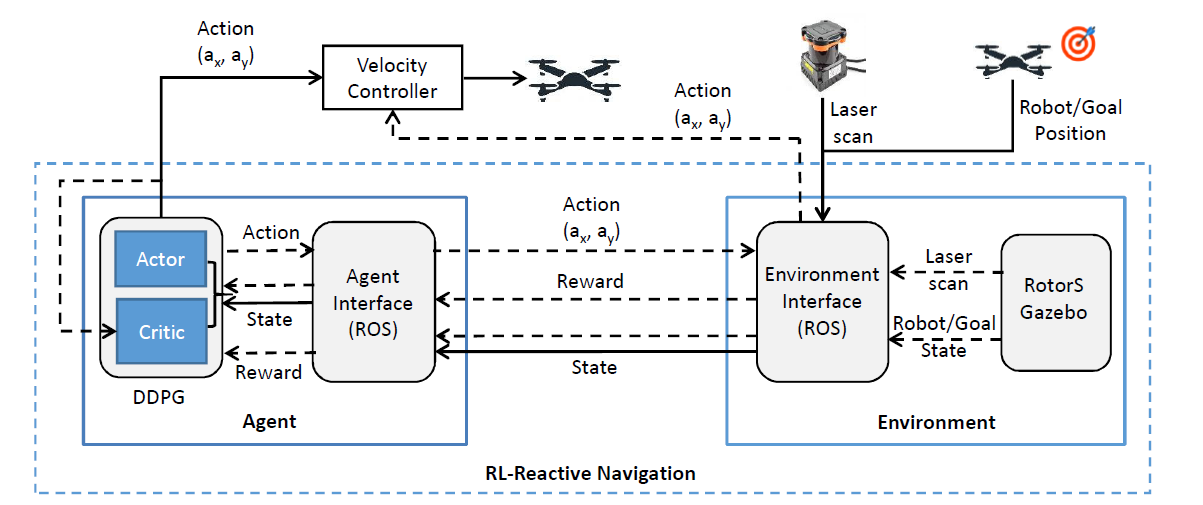
\includegraphics[width=\textwidth]{imagenes/cap2/drone-architecture.png}
    \caption{Arquitectura propuesta para el sistema de navegación reactivo original \cite{Sampedro2018}.}
    \label{fig:chap2-drone}
\end{figure}

Ahora bien, existen diferencias destacables entre la propuesta original y el trabajo descrito en esta memoria:

\begin{itemize}
	\item \textbf{Movimientos del agente:} La propuesta original utiliza como agente a un dron multirotor, capaz de navegar por el aire (aunque se mantiene a una altura constante) y de realizar movimiento omnidireccional. En cambio, el trabajo desarrollado utiliza un robot terrestre (susceptible a obstáculos en el suelo) incapaz de movimiento omnidireccional, siendo necesario el giro del agente para poder esquivar obstáculos y desplazarse.
	\item \textbf{Sensores del agente:} Mientras que la propuesta original utiliza un conjunto de láseres para percibir su entorno, el trabajo desarrollado propone un agente con una única cámara de profundidad frontal. Si bien el conjunto de láseres resulta más caro que una cámara de profundidad, también ofrece un ángulo de visión mayor de los obstáculos del entorno.
	\item \textbf{Complejidad del entorno:} La propuesta original entrena al agente en entornos de interior simples (contando con espacios simples con obstáculos dispersos), frente a los entornos usados por el trabajo desarrollado (siendo recreaciones del interior de domicilios, incluyendo topografías más complejas con cuartos y una mayor cantidad de obstáculos y ruido).
\end{itemize}

